\documentclass[12pt]{article}
\usepackage{graphicx} % Required for inserting images
\usepackage{geometry}
\geometry{a4paper, margin=2.5cm}
\usepackage[T1]{fontenc}
\usepackage{palatino}
\usepackage{amsmath, amssymb}
\usepackage{array}
\usepackage{titling}
\usepackage{subcaption}

\setlength{\droptitle}{-5em}
\preauthor{\begin{center}\large\vspace{0.5em}}
\postauthor{\end{center}\vspace{-0.5em}}

\title{
    {\scshape  Part IIB Revision Notes} \\ 
    \vspace{0.5em}
    \textbf{4F14: Computer Systems}}
\author{Qianshuo (Harry) Ye}
\date{April 2026}
\usepackage{parskip}
\begin{document}
\maketitle

\section{Introduction}
\textbf{Central processing unit (CPU):} Components of the CPU are:
\begin{itemize}
    \item \textit{Control unit:} Fetches instructions from main memory and determines their type. Coordinates data flow around the CPU during instruction execution.
    \item \textit{Arithmetic logic unit (ALU):} Performs simple arithmetic and logic functions on data within the CPU.
    \item \textit{Registers:} Small, high speed memory used to store temporary results and control information.
\end{itemize}

\textbf{Fetch-decode-execute cycle:} Instructions are executed in the follow cycle:
\begin{enumerate}
    \item \textit{Fetch} next instruction from main memory.
    \item Increment the PC to point to the next instruction.
    \item \textit{Decode} instruction.
    \item If the instruction uses data from memory, calculate the relevant address and fetch the data.
    \item Fetch data from memory.
    \item \textit{Execute} the instruction.
    \item Store results.
\end{enumerate}

\textbf{Memory addressing:}
\begin{itemize}
    \item \textit{Byte-addressable:} Each address refers to an 8-bit quantity (a byte).
    \item \textit{Word:} A unit of data manipulated by the CPU (the size of the register). (4 bytes for a 32-bit processor)
\end{itemize}
$$
\text{word address} = \left\lfloor \frac{\text{byte address}}{4} \right\rfloor
$$

\textbf{Byte ordering:} Big endian (most significant byte stored at the lowest address) vs little endian (least significant byte stored at the lowest address).

\textbf{Magnetic disks:} 
\begin{itemize}
    \item Glass/ceramic platters coated in thin film magnetic media rotate at high speed.
    \item Data is read/written by electromagnetic heads that float above both surfaces of the platters.
    \item Each surface is divided into $\sim$ 280,000 \textit{tracks}.
    \item The collection of tracks under the heads at a given time is called a \textit{cylinder}.
    \item Each track is divided into $\sim$ 850-2600 \textit{sectors}, which are the smallest units that can be read/written.
    \item The time to read or write a sector of data to or from the disk is
    $$\text{access time} = \text{seek time} + \text{rotational latency} + \text{transfer time} + \text{controller overhead}$$
    \begin{itemize}
        \item \textit{Seek time:} Time taken to move the heads to the right cylinder.
        \item \textit{Rotational latency:} Time taken for the right sector to rotate under the head.
        \item \textit{Transfer time:} Time taken to read/write the data from/to the disk.
        \item \textit{Controller overhead:} Time taken by the disk controller to process the request.
    \end{itemize}
\end{itemize}

\textbf{Performance measurement:} \textit{Execution time} is the time fo perform a single job, while \textit{throughput} is the total work done per unit time. The run-time can be broken down as:
$$
\text{time} = \text{instructions} \times \frac{\text{clock cycles}}{\text{instruction}} \times \frac{\text{seconds}}{\text{clock cycle}}
$$
To improve performance for a fixed instruction set:
\begin{enumerate}
    \item Reduce the number of instructions per program.
    \item Reduce the number of clock cycles per instruction.
    \item Reduce the clock cycle time.
\end{enumerate}

\textit{FLOPS} (floating point operations per second) is a common performance metric.

\textbf{Amdahl's law:} ``Make the common case fast.''
$$
t_\text{new} = t_\text{old} \times \left[ (1 - f) + \frac{f}{s} \right]
$$
where $f$ is the fraction of execution time affected by the improvement and $s = \frac{t_\text{prog, old}}{t_\text{prog, new}}$ is the speedup of the improved portion.

\section{Instruction Set Architecture}
\textbf{Instruction:} An \textit{instruction = opcode + operands}.
\begin{itemize}
    \item \textit{Opcode:} Type of operation to perform.
    \item \textit{Operands:} Data to be operated on.
\end{itemize}

\textbf{Classification of ISAs:}
\begin{itemize}
    \item \textit{Stack ISA}: Operands are taken from the stack. e.g. \texttt{add} does stack(1) $\leftarrow$ stack(2) + stack(3)
    \item \textit{Accumulator ISA:} One operand is implicitly taken from the accumulator (a special register). e.g. \texttt{lda 0xE000} does accumulator $\leftarrow$ word at E000.
    \item \textit{General purpose register ISA:} All operands are explicitly declared, either registers or memory. The key parameters are: the \textit{number of operands} per ALU instruction and the \textit{maximum number of memory references} in ALU instructions.
\end{itemize}

\textbf{MIPS ISA:} A \textit{load-store} architecture (only load and store instructions can access memory) with fixed-size 32-bit instructions and 32 general purpose registers. The operands can be registers or memory words.
\begin{center}
    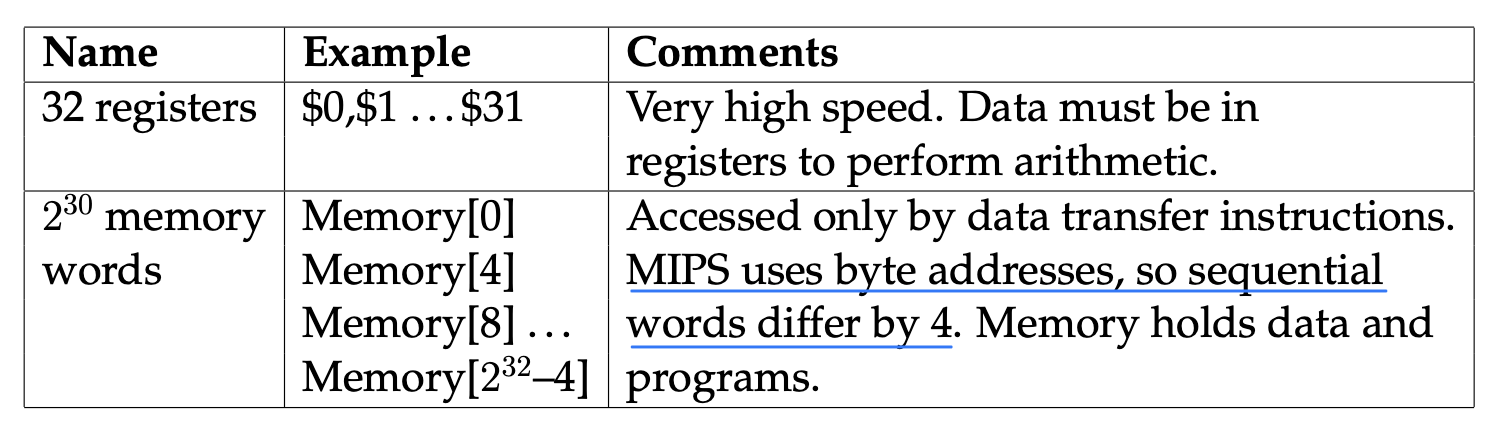
\includegraphics[width=0.7\textwidth]{figures/4F14/MIPS_operand.png}
\end{center}

\textbf{Assembly language:} The symbolic representation of instructions, can be translated into \textit{machine language} (executable code) by an assembler (also accepts \textit{pseudo-instructions}).

\textbf{R-format instruction:}
\begin{center}
    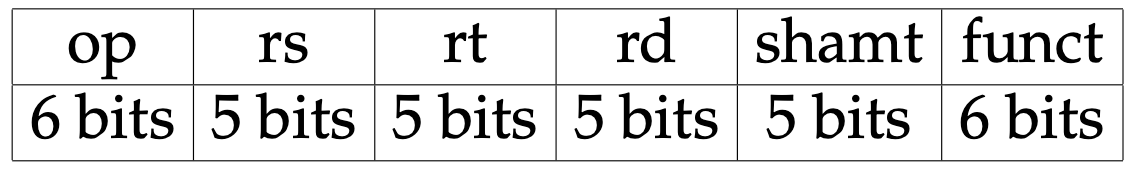
\includegraphics[width=0.4\textwidth]{figures/4F14/R-format.png}
\end{center}
\begin{itemize}
    \item op = operation of the instruction
    \item rs = first register source operand
    \item rt = second register source operand
    \item rd = register destination operand
    \item shamt = shift amount (for shift instructions)
    \item funct = selects variant of operation in op field
\end{itemize}
Examples:
\begin{itemize}
    \item Add: \texttt{add \$8,\$17,\$18} means \$8 = \$17 + \$18. The machine language in decimal is [0, 17, 18, 8, 0, 32].
    \item Subtract: \texttt{sub \$8,\$17,\$18} means \$8 = \$17 - \$18. 
    \item Move (pseudo): \texttt{move \$8,\$18} means \$8 = \$18. It is equivalent to \texttt{add \$8,\$0,\$18}.
    \item Set on less than: \texttt{slt \$1,\$2,\$3} means if \$2 < \$3, then \$1 = 1; else \$1 = 0.
    \item Jump register: \texttt{jr \$8} means jump to the address in register \$8 (PC = \$8). The machine language in demcimal is [0, 8, 0, 0, 0, 8].
\end{itemize}

\textbf{I-format instruction:}
\begin{center}
    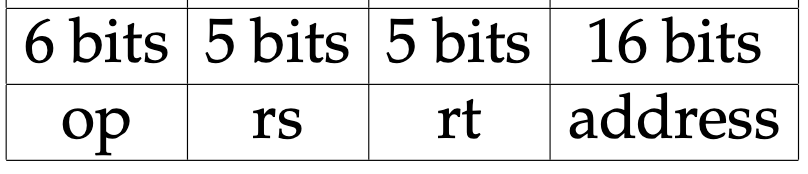
\includegraphics[width=0.3\textwidth]{figures/4F14/I-format.png}
\end{center}
The \textit{addressing modes} specifies how an instrunction accesses its operands:
\begin{itemize}
    \item \textit{Register:} operand is a register.
    \item \textit{Immediate:} operand is a constant value.
    \item \textit{Displacement/base:} operand is in memory, the address is the sum of a register and an offset in the instruction.
    \item \textit{PC-relative:} operand is in memory, the address is the sum of the program counter and a constant in the instruction.
\end{itemize}

Examples:
\begin{itemize}
    \item Load word: \texttt{lw \$15,100(\$2)} means \$15 = mem[\$2 + 100]. The machine language in demcimal is [35, 2, 15, 100].
    \item Save word: \texttt{sw \$15,100(\$2)} means mem[\$2 + 100] = \$15.
    \item Branch if equal: \texttt{beq \$19, \$20, L1} means if \$19 == \$20, then PC = PC + 4 + 4 * L1 (4* since the 16-bit address is a \textit{word} offset). The machine language in decimal is [4, 19, 20, L1].
    \item Branch if not equal: \texttt{bne \$19, \$20, L1} means if \$19 != \$20, then PC = PC + 4 + 4 * L1.
    \item Addi: \texttt{addi \$19, \$19, 4} means \$19 = \$19 + 4. The machine language in decimal is [8, 19, 19, 4], where 4 is the 16-bit \textit{immediate}.
\end{itemize}

\textbf{J-format instruction:} 
\begin{center}
    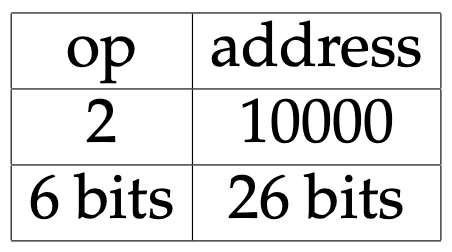
\includegraphics[width=0.15\textwidth]{figures/4F14/J-format.png}
\end{center}
The 26-bit address is a \textit{word} address, so it is effectively a 28-bit byte address (can address up to 256 MiB). The program counter is 32-bit, so only the lower 28 bits of the PC are replaced.

Examples:
\begin{itemize}
    \item Jump instruction: \texttt{j exit} means jump to address with label \texttt{exit}. The machine language in decimal is [2, 10000].
    \item Jump and link: \texttt{jal A} means call procedure A and save the return address (PC + 4) in register \$31, so it is possible to return after a procedure. If a procedure calls another procedure, the return address must be stored on the stack (fills top-down in MIPS), where the address of the bottom of the stack is in register \$29.
\end{itemize}

\textbf{Parameter passing:} The first 4 parameters are passed in registers \$4 to \$7, and the rest are passed on the stack. If another procedure is called, or registers are used as scratch space, the registers need to be saved and restored, with two conventions:
\begin{itemize}
    \item \textit{Caller save:} The calling routine saves the register on the stack.
    \item \textit{Callee save:} The called routine saves the register on the stack.
\end{itemize}

\textbf{MIPS data sheet terms:}
\begin{itemize}
    \item \textit{Zero-extend:} Fill the upper bits with 0s.
    \item \textit{Sign-extend:} Take the most significant bit (the sign bit) of the smaller number and fill the upper bits with it.
    \item \textit{Traps:} CPU will trigger an exception or interrupt. The address of the offending instruction is stored in a register and the computer jumps to a predefined address to invoke the appropriate handling routine.
\end{itemize}

\section{ALU Design}
\textbf{Full adder:} Simplified boolean expression for the Sum and CarryOut:
\begin{align*}
    \text{CarryOut} &= \text{a.CarryIn} + \text{b.CarryIn} + \text{a.b} \\
    \text{Sum} &= \text{a}.\overline{\text{b}}.\overline{\text{CarryIn}} + \overline{\text{a}}.\text{b}.\overline{\text{CarryIn}} + \overline{\text{a}}.\overline{\text{b}}.\text{CarryIn} + \text{a.b.CarryIn}
\end{align*}

\textbf{1-bit ALU:} Can perform AND, OR, addition, subtraction, and \texttt{slt}. For subtraction, set Binvert and CarryIn of the LSB to 1. For \texttt{slt}, use the Less input.

3 control lines switch the multiplexors inside the 1-bit ALU: 1 line for Binvert, 2 lines for Operation.
\begin{center}
    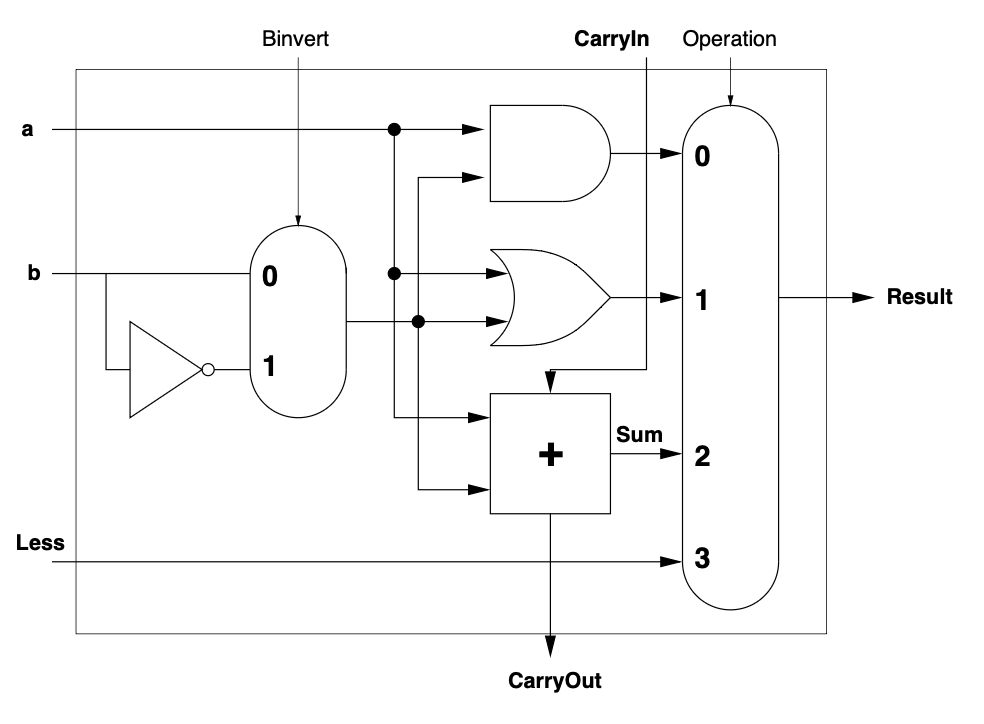
\includegraphics[width=0.4\textwidth]{figures/4F14/1-bit_ALU.png}
\end{center}

\textbf{Ripple-carry 32-bit ALU:} Connect 32 1-bit ALUs, propagating the carry from one bit to the next. \texttt{slt} is performed by subtracting b from a and passing the Less signals to the Result line (Result 0 = 1 if a < b, all other results = 0).
\begin{center}
    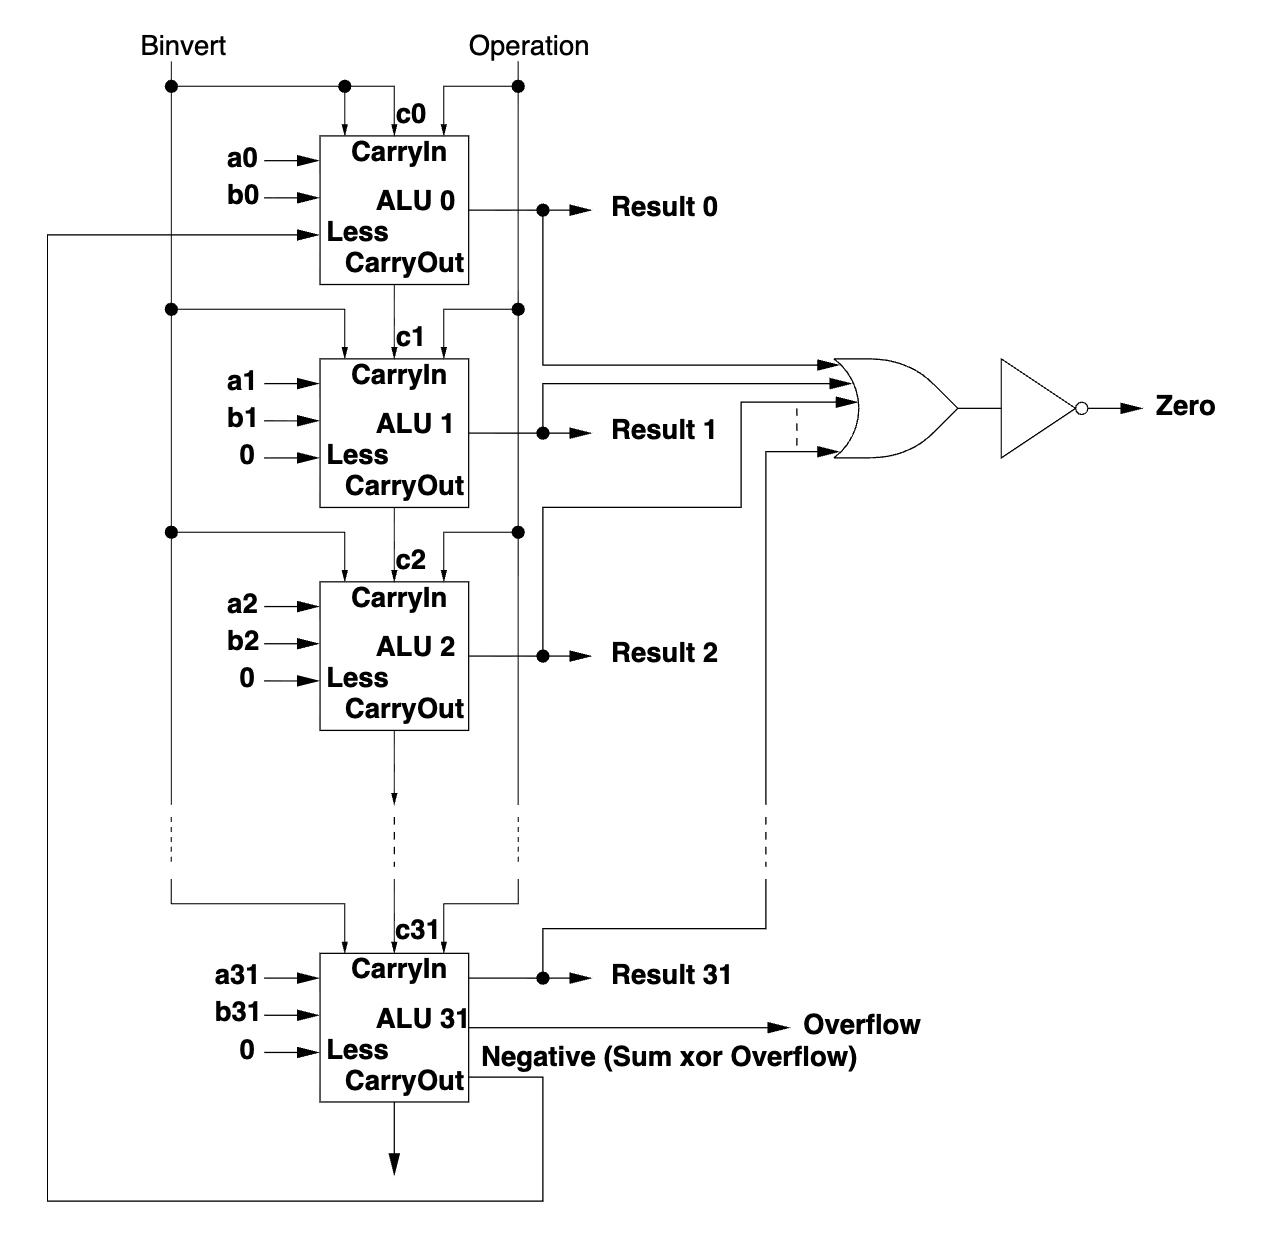
\includegraphics[width=0.5\textwidth]{figures/4F14/32-bit_ALU.png}
\end{center}

\textbf{Carry-lookahead 16-bit ALU:} Anticipate the CarryIn signal wihout waiting for it to propagate through the adder. Define:
\begin{itemize}
    \item \textit{Generate:} gi = ai.bi (carry generated by bit i)
    \item \textit{Propagate:} pi = ai + bi (carry propagated by bit i)
\end{itemize}
It follows that c(i+1) = ai.ci + bi.ci + ai.bi = gi + pi.ci.

4-bit carry-lookahead adder:
\begin{itemize}
    \item[] c1 = g0 + p0.c0
    \item[] c2 = g1 + p1.c1 = g1 + p1.g0 + p1.p0.c0
    \item[] c3 = g2 + p2.c2 = g2 + p2.g1 + p2.p1.g0 + p2.p1.p0.c0
    \item[] c4 = g3 + p3.c3 = g3 + p3.g2 + p3.p2.g1 + p3.p2.p1.g0 + p3.p2.p1.p0.c0
\end{itemize}
Connect 4 4-bit adders using a higher level of carry-lookahead (propagate if all 4 bits propagate, generate if any bit generates):
\begin{itemize}
    \item[] P0 = p0.p1.p2.p3, G0 = g3 + p3.g2 + p3.p2.g1 + p3.p2.p1.g0
    \item[] P1 = p4.p5.p6.p7, G1 = g7 + p7.g6 + p7.p6.g5 + p7.p6.p5.g4
    \item[] P2 = p8.p9.p10.p11, G2 = g11 + p11.g10 + p11.p10.g9 + p11.p10.p9.g8
    \item[] P3 = p12.p13.p14.p15, G3 = g15 + p15.g14 + p15.p14.g13 + p15.p14.p13.g12
\end{itemize}
The carry-in signals are:
\begin{itemize}
    \item[] C1 = G0 + P0.c0
    \item[] C2 = G1 + P1.C1 = G1 + P1.G0 + P1.P0.c0
    \item[] C3 = G2 + P2.C2 = G2 + P2.G1 + P2.P1.G0 + P2.P1.P0.c0
    \item[] C4 = G3 + P3.C3 = G3 + P3.G2 + P3.P2.G1 + P3.P2.P1.G0 + P3.P2.P1.P0.c0
\end{itemize}
Result is produced after 9 gate delays (each sum-of-product = 2 gate delays). For an $n$-bit adder, if $m$ carrying signals are generated at each level, $\log_m n$ levels are needed.
\begin{center}
    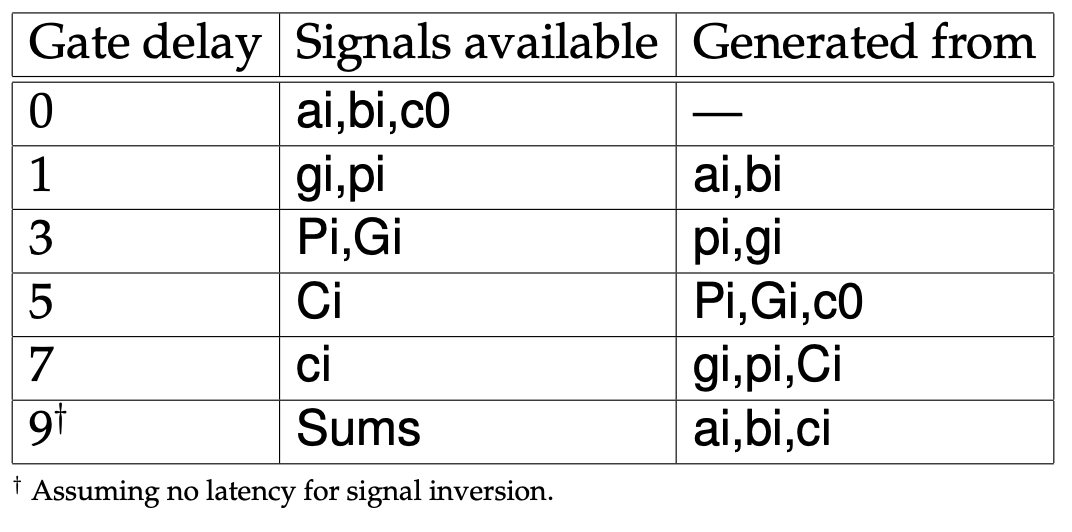
\includegraphics[width=0.4\textwidth]{figures/4F14/cla_delay.png}
    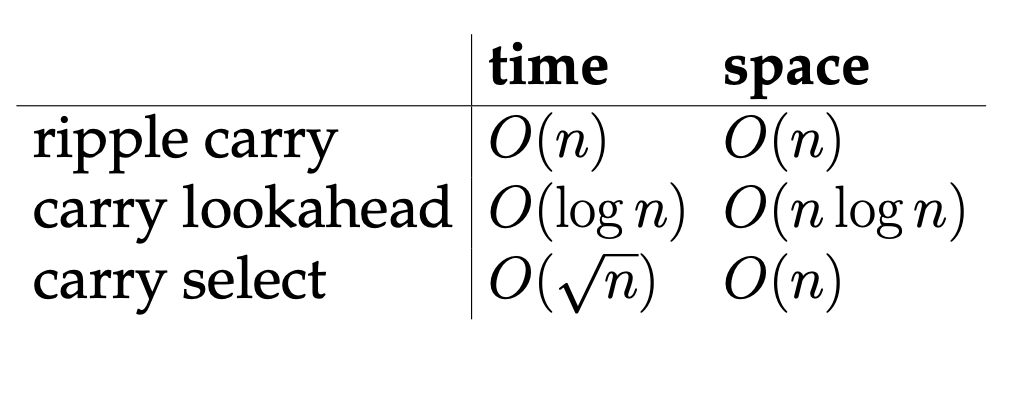
\includegraphics[width=0.4\textwidth]{figures/4F14/ALU_complexity.png}
\end{center}

\section{Datapaths and Pipelining}
\textbf{Datapath:}
The \textit{register file} has 3 5-bit inputs to select the 2 registers to be read and 1 register to be written. It also has 2 32-bit outputs and 1 32-bit input for reading and writing data.
\begin{center}
    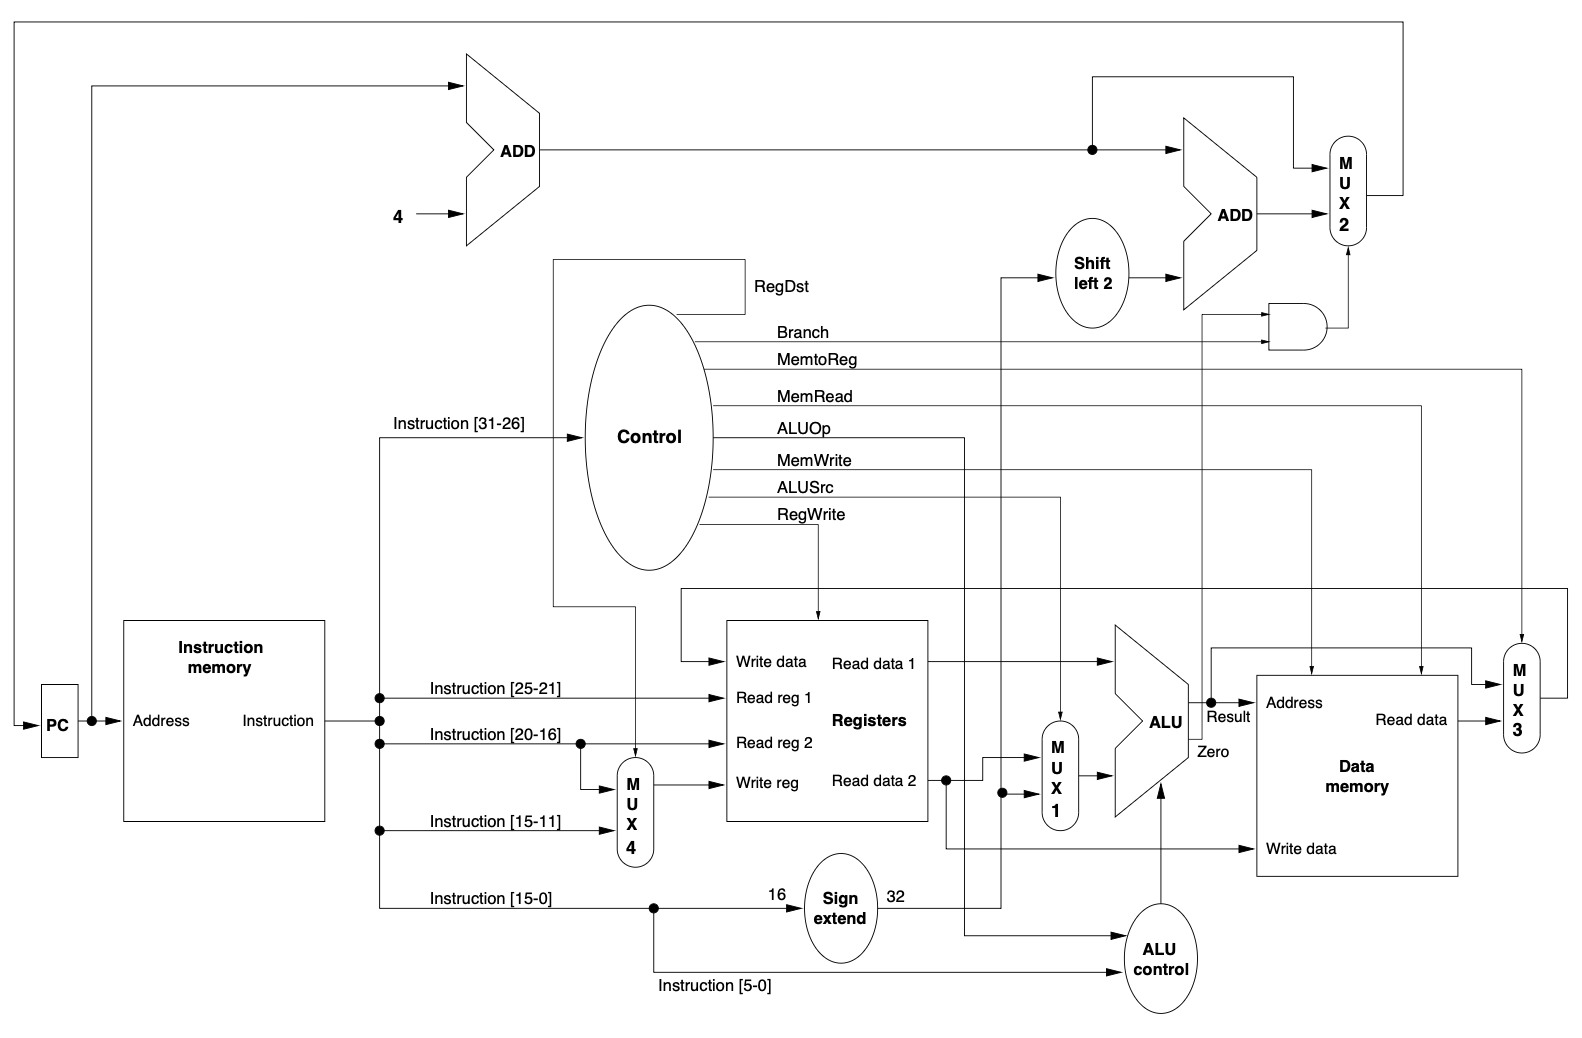
\includegraphics[width=0.90\textwidth]{figures/4F14/full_datapath.png}
\end{center}
The multiplexors MUX1, MUX2 and MUX3 select signals based on the instruction. Bits 26-31 of the instruction always define the operation class. For R-format instruction, bits 0-5 defines the ALU operation.

\textbf{Datapath control:}
\begin{center}
    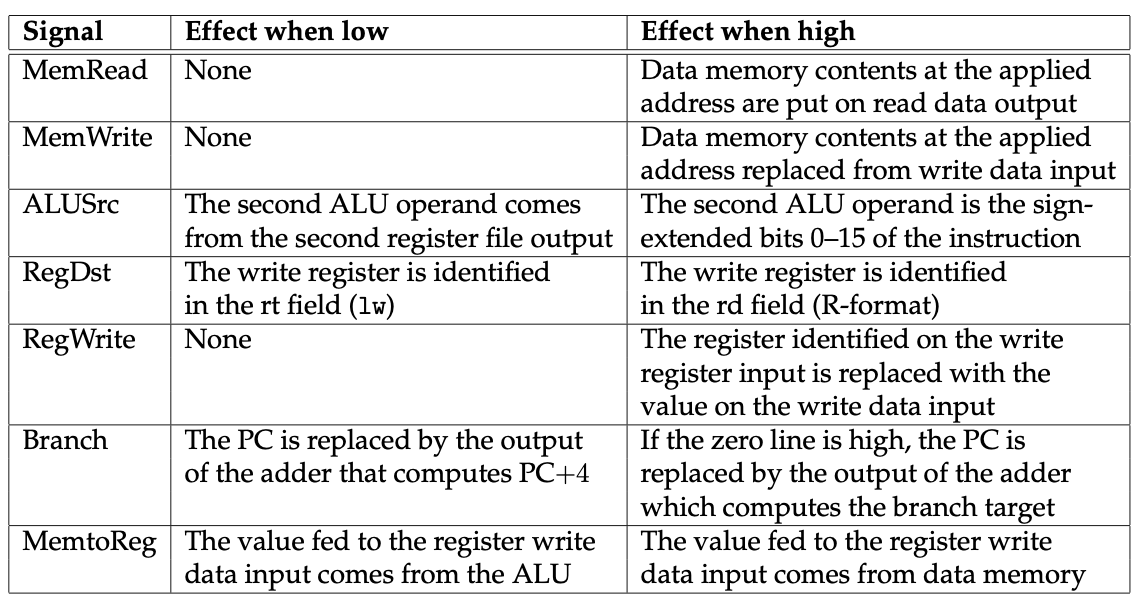
\includegraphics[width=0.6\textwidth]{figures/4F14/datapath_control.png}
    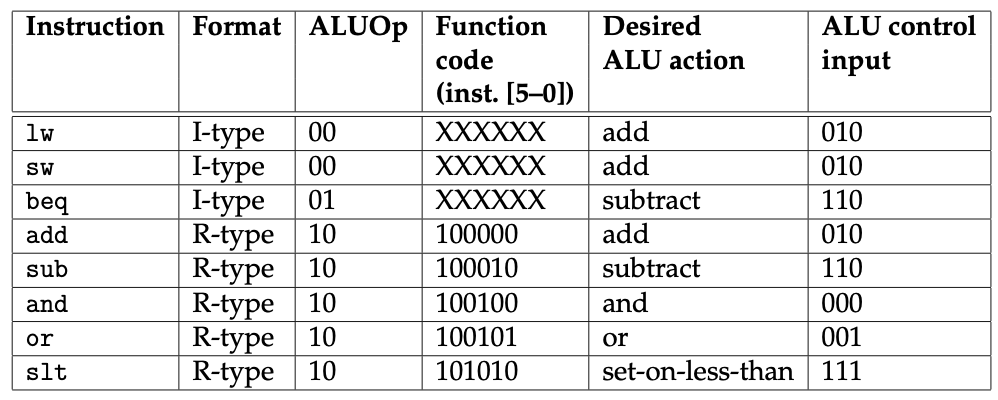
\includegraphics[width=0.6\textwidth]{figures/4F14/ALU_control.png}
\end{center}
A truth table of the control signals for each instruction (bits 0-5 and 26-31) can be implemented in \textit{ROM or Programmable Logic Array}.

\textbf{Multiple clock-cycle datapath:} Instructions are broken up into steps, with each step taking one cycle. The control is implemented using a \textit{state machine} consisting of a set of states and a function to find the next state given the current state, and a set of outputs (control signal).
Complex control signals can be instead implemented using a \textit{microprogram}.

\textbf{Pipelining:} Split the instruction execution cycle into 5 \textit{pipe stages}:
\begin{enumerate}
    \item IF: Instruction fetch
    \item ID: Instruction decode and register fetch
    \item EX: Execution and effective address calculation
    \item MEM: Memory access
    \item WB: Write back to register file
\end{enumerate}
For a large number of instructions, the speed-up approaches 4:1. Extra \textit{pipeline registers} stores the result from one pipe stage so that it can be used by the next. 
\begin{center}
    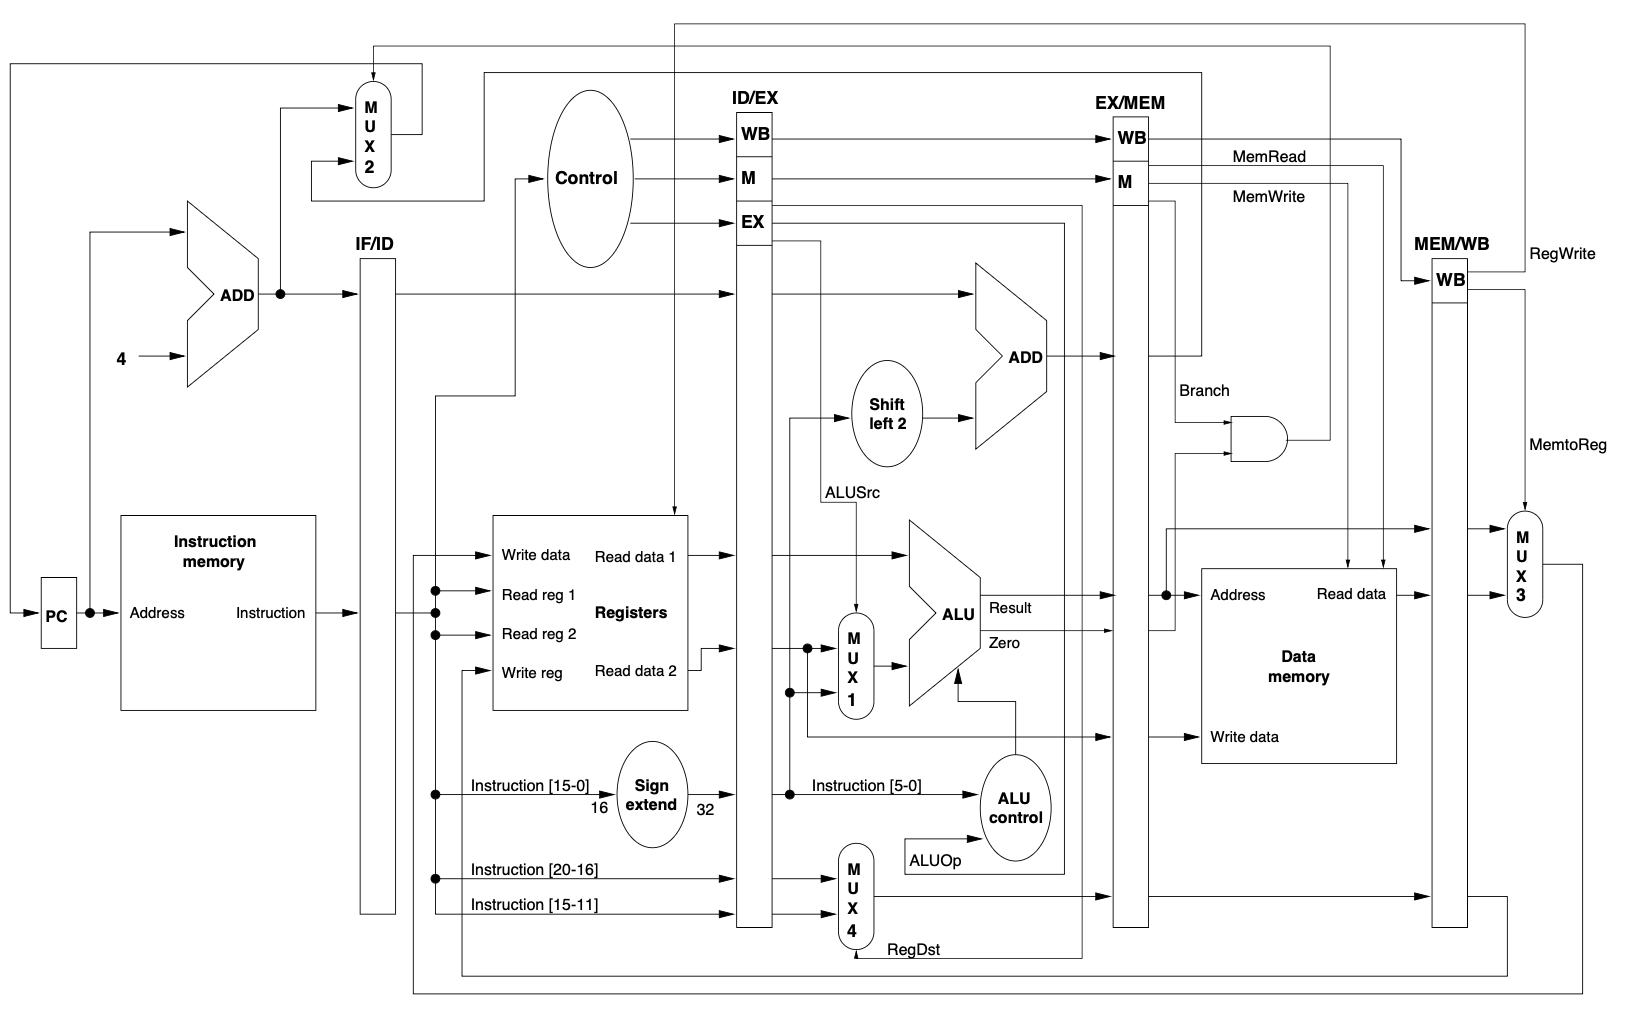
\includegraphics[width=0.95\textwidth]{figures/4F14/full_pipeline.png}
\end{center}

\textbf{Data hazards:} Data hazards occur when a value required in a register is not valid because a previous instruction has not yet updated it. Solutions include:
\begin{itemize}
    \item \textit{Stall:} Stages of dependent instructions are not executed until value is available. Creates \textit{bubbles} into the pipeline and reduces the computer's efficiency. Implemented by adding a \textit{hazard detection unit}.
    \item \textit{Data forwarding:} Forward values directly to the ALU inputs, bypassing the register write-back. Implemented by adding multiplexors to the inputs of the ALU and supplying suitable control lines.
    
    The forwarding unit compares the registers that have just been read with any registers about to be written by the two downstream instructions (at stages MEM and WB). If there is a match, MUXA and/or MUXB are set to ignore the value read from the register file and instead use the appropriate forwarded value. 
    \begin{center}
        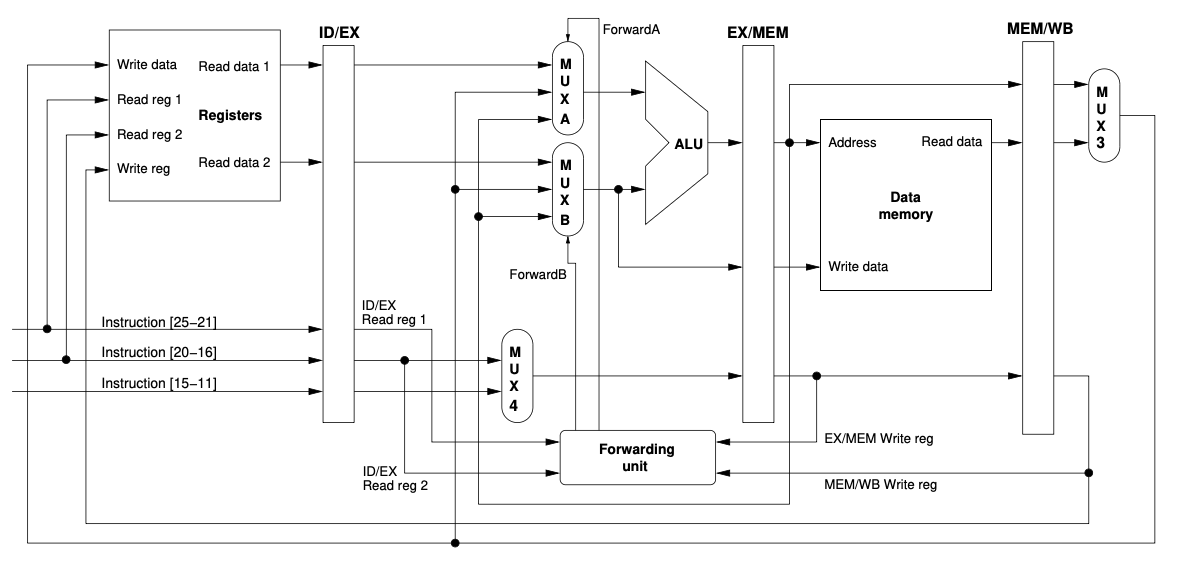
\includegraphics[width=0.8\textwidth]{figures/4F14/data_forwarding.png}
    \end{center}
    Not working for \texttt{lw} as data is read from memory and required at the ALU at the same time. Can be solved by stalling or requiring the software to follow \texttt{lw} with an instruction indepedent of the load -- \textit{delayed load}.
\end{itemize}
\begin{center}
    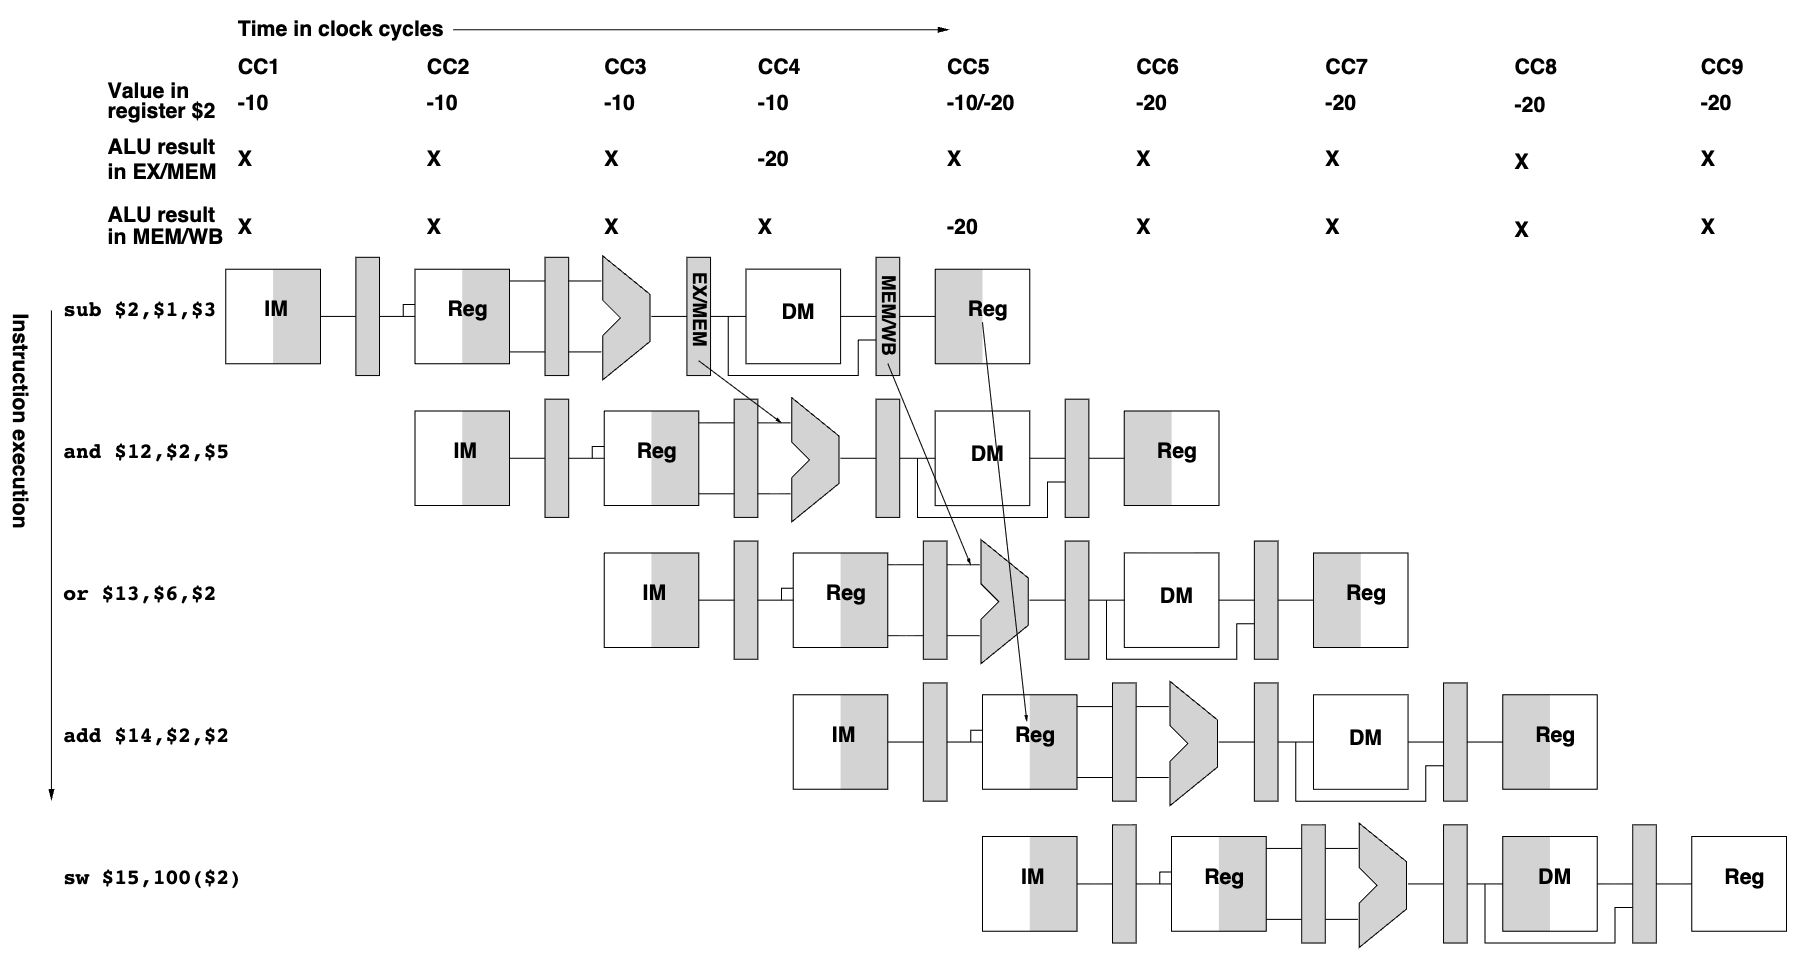
\includegraphics[width=0.8\textwidth]{figures/4F14/data_forwarding_pipeline.png}
\end{center}

\textbf{Branch hazards:} The address of the next instruction is not known until the branch instruction reaches stage 4 of the pipeline. Solutions include:
\begin{itemize}
    \item Always stall on branches.
    \item Assume branch not taken and execute next instructions. If the branch is actually taken, flush the pipeline and discard the partial results, resuming execution at the branch target address.
    \item Predict the branch outcome.
    \item \textit{Delayed branches:} The instruction following the branch instruction is always executed (independent of the branch outcome)
    \texttt{\\branch instruction \\ next instruction \\ branch to target if branch taken}
\end{itemize}

\textbf{Superpipline and superscalar:} Superpiplining split the pipe stages into smaller stages with shorter clock cycles. Superscalar allows multiple instructions to be executed at the same clock cycle.

\section{Memory Systems}
\textbf{Memory hierarchy:} At each level of the hierarchy, the information stored is a subset of that lower down, based on the principle of locality:
\begin{itemize}
    \item \textit{Temporal locality:} if an item is referenced, it tends to be referenced again soon (loops, local variables).
    \item \textit{Spatial locality:} if an itme is referenced, items with nearby addresses will tend to be referenced soon (instructions, data in arrays).
\end{itemize}
A \textit{hit} occurs if requested data is present in an upper level, otherwise a \textit{miss}. Aim for high hit rate and low miss penalty.
\begin{center}
    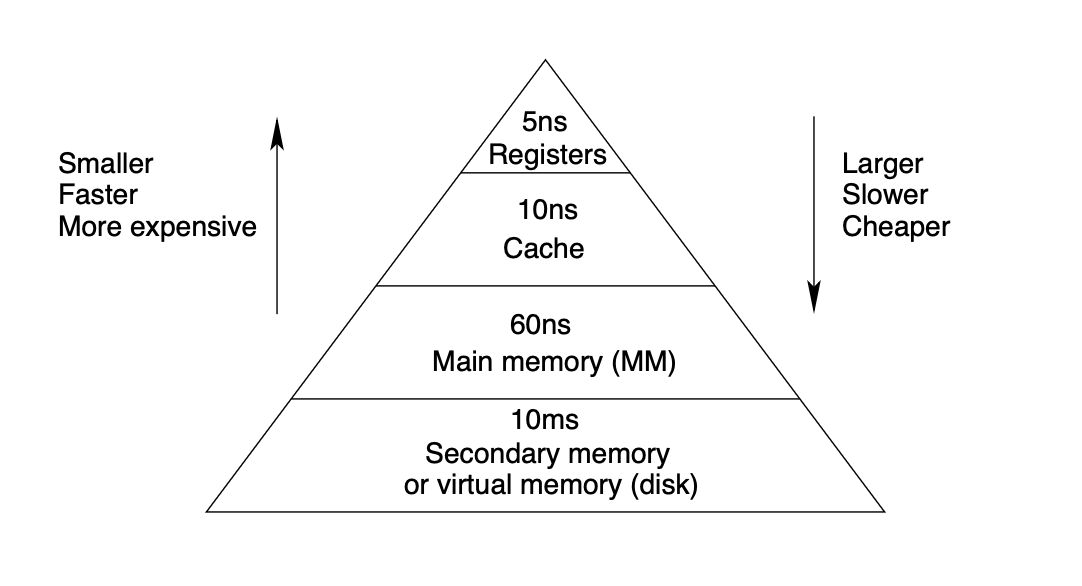
\includegraphics[width=0.5\textwidth]{figures/4F14/memory_tier.png}
\end{center}

\textbf{Cache:} Words in a cache are arranged in \textit{blocks}. If a word is not in the cache, the block containing the word will be loaded from main memory.

\textbf{Direct-mapped cache:} For every main memory address, there is a unique cache location (identified by an \textit{index}) that can hold it. 
$$
\text{index} = \underbrace{\left\lfloor \frac{\text{byte address}}{\text{\# bytes per block}} \right\rfloor}_{\text{block address}} \mod \text{ \# blocks in cache}
$$
\begin{center}
    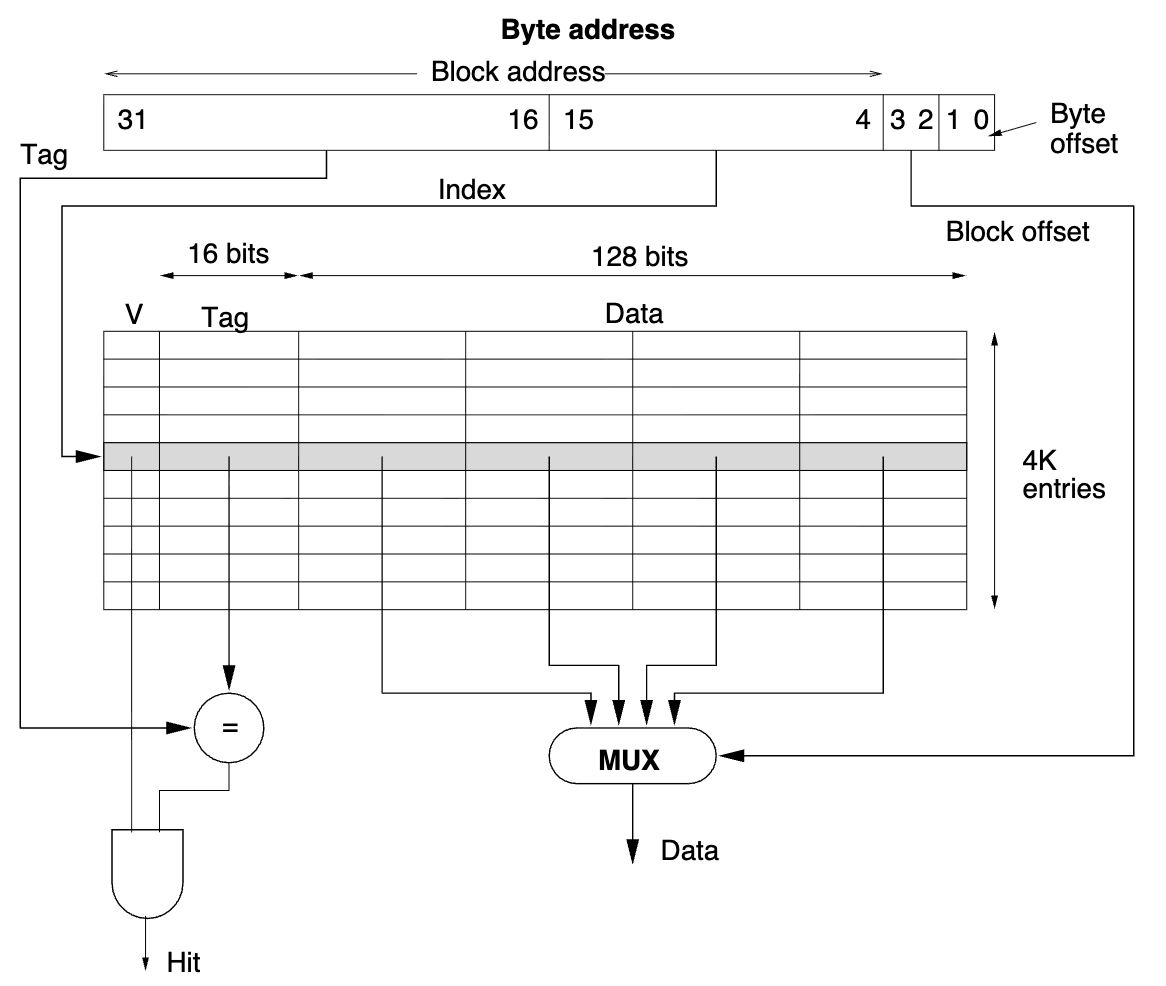
\includegraphics[width=0.5\textwidth]{figures/4F14/direct_mapped_cache.png}
\end{center}
To reference a word in the cache:
\begin{itemize}
    \item 12-bit \textit{index} identifies the block in the cache.
    \item 16-bit \textit{tag} identifies the block in main memory, compared with the stored tag to check for a hit. (1 cache block can correspond to $2^{16}$ blocks in main memory)
    \item 2-bit \textit{block offset} identifies the word within the block.
    \item The \textit{valid bit} is set low on start-up.
\end{itemize}
To handle a cache miss, stall the entire machine and do:
\begin{enumerate}
    \item Reset the PC to PC - 4.
    \item Instruct main memory to read the requested block and wait for completion.
    \item Write the data and tag into the cache and set the valid bit to 1.
    \item Restart the pipeline, which will fetch the instruction again and get a hit this time.
\end{enumerate}

\textbf{Cache writes:} Update the main memory when the cache is updated, two approaches available:
\begin{itemize}
    \item \textit{Write through:} data is written to the cache and also the main memory. \textit{Write buffers} can be used to avoid stalling. \\
    Advantages: read misses are cheaper since they do not require a write to main memory \& easier to implement.
    \item \textit{Write back:} data is written only to the cache, and the modified cache block is written to main memory only when it is replaced. \\
    Advantages: words are written at cache rather than main memory speed \& multiple writes to a block require only one write to main memory. 
\end{itemize}

\textbf{Associative caches:}
\begin{itemize}
    \item \textit{Fully associative cache:} A memory block can reside anywhere in the cache. A full search of the cache is needed to determine if a word is present.
    \item \textit{Set associative cache:} A memory block can reside in a number of locations in a unique set. Only a search within the set is needed. The index of the set is (block address) mod (\# sets in cache).
\end{itemize}
\begin{center}
    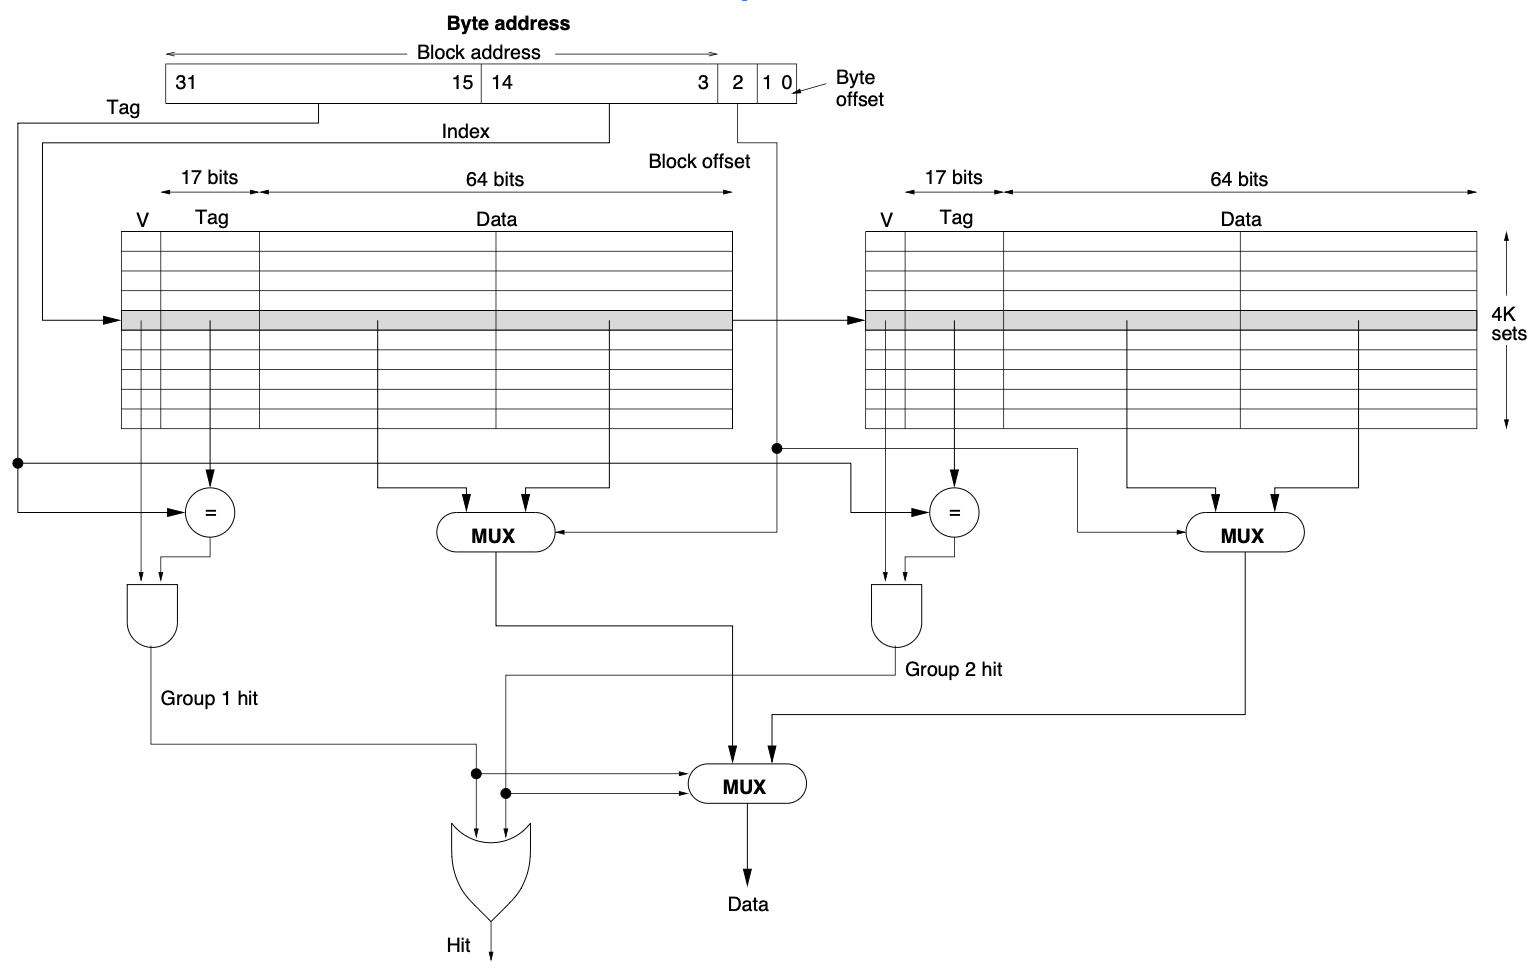
\includegraphics[width=0.8\textwidth]{figures/4F14/set_associative.png}
\end{center}

\textbf{Block replacement:} Two common strategies:
\begin{itemize}
    \item \textit{Random:} Randomly select a block to replace.
    \item \textit{Least recently used (LRU):} Replace the block that has been unused for the longest time. Efficient at larger degrees of associativity.
\end{itemize}

\textbf{Cache performance:}
\begin{itemize}
    \item Execution time = (CPU execution cycles + memory stall cycles) $\times$ clock cycle time
    \item Memory stall cycles = \# instructions $\times$ misses per instruction $\times$ miss penalty 
\end{itemize}
To improve performance, reduce the miss rate by using a multi-level cache (small, fast, primary, low associativity cache + large secondary, high associativity cache), or reduce the miss penalty by incerasing the bandwidth to main memory (e.g. use a wider bus).

\textbf{Virtual memory:}
\begin{itemize}
    \item Allows the total amount of memory available to a program to exceed the physical amount of main memory.
    \item Allows main memory to be shared between multiple programs on the same machine, with each program having its own address space and is protected from other programs.
\end{itemize}
Virtual addresses are used and translated into physical address by the operating system.
The main memory and virtual memory are divided into \textit{pages}.

Main memory acts as a cache for virtual memory with a block size of one page. A \textit{page fault} corresponds to a cache miss.

The location of pages (fully associative) is stored in a \textit{page table} indexed by the virtual page number and contains the physical page number. Each running program has its own page table. A \textit{page table register} points to the start of the page table. For each page table entry, a valid bit determines whether the page is in memory.

Write-back is used, with a \textit{dirty bit} to indicate whether the page has been modified.

\begin{center}
    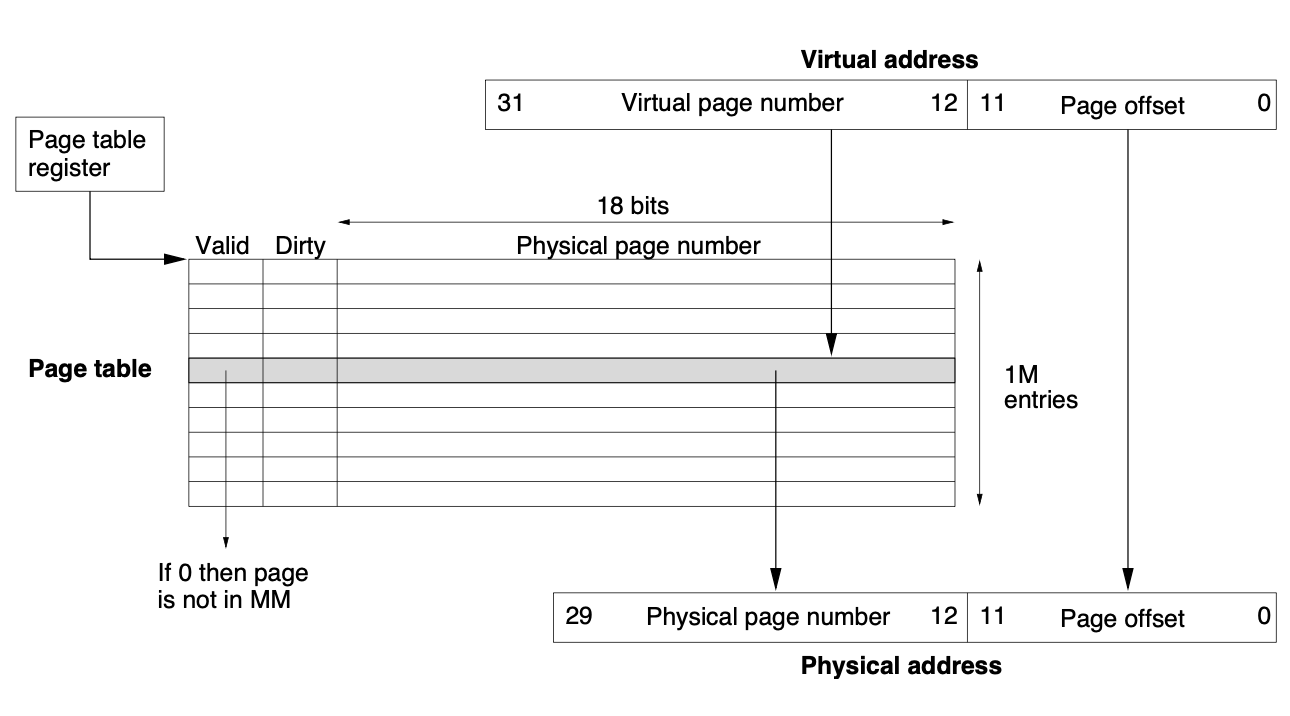
\includegraphics[width=0.6\textwidth]{figures/4F14/page_table.png}
\end{center}

\textbf{Translation lookaside buffer (TLB):} A special, fast cache to store recently used translations. The TLB only caches part of the page table that point to main memory, often fully associative with random placement. Each entry contains:

\begin{itemize}
    \item Tag = full virtual page number (fully associative) or part of the virtual page number (not fully associative, with the rest of the virtual page number as index).
    \item Data = physical page number + dirty bit.
\end{itemize}

Write-back is used to ensure the dirty bits are kept up to date.

On a TLB miss, if the page is in main memory, the TLB entry is updated from the page table and the translation retired. Otherwise, a page fault is generated.

\begin{center}
    \includegraphics[width=0.6\textwidth]{figures/4F14/tlb.png}
\end{center}

\textbf{Process:} The state of a program defined by the page table, the PC and the other registers. When a process switch occurs, it is necessary to either flush the TLB or extend the virtual address with a process identifier to distinguish entries from different processes.

\section{Interfacing to I/O Devices}
\textbf{Measuring I/O performance:}
\begin{itemize}
    \item \textit{Bandwidth:} How much data can flow through the system per second?
    \item \textit{Latency:} How long does it take to initialise an I/O process?
\end{itemize}

\textbf{Bus:} A bus is a shared communication link which uses one set of wires to connect multiple subsystems. There are two main classes of buses:
\begin{itemize}
    \item \textit{Processor-memory:} short, high performance, matched to memory system.
    \item \textit{I/O:} long, wide range of data rates, used to connect diverse devices.
\end{itemize}
And two schemes for bus communications:
\begin{itemize}
    \item \textit{Synchronous:} control lines include a clock signal, all transfers are relative to the clock. Buses run at the speed of the slowest device.
    \item \textit{Asynchronous:} no clock, every transfer is acknowledged by the recipient before more data is sent. Can be long since there is no clock skew.
\end{itemize}

\textbf{Handshaking:} Three control lines: \textit{ReadReq} (indicate a read request), \textit{DataRdy} (indicate that data is available), \textit{Ack} (acknowledge the ReadReq or DataRdy).
\begin{center}
    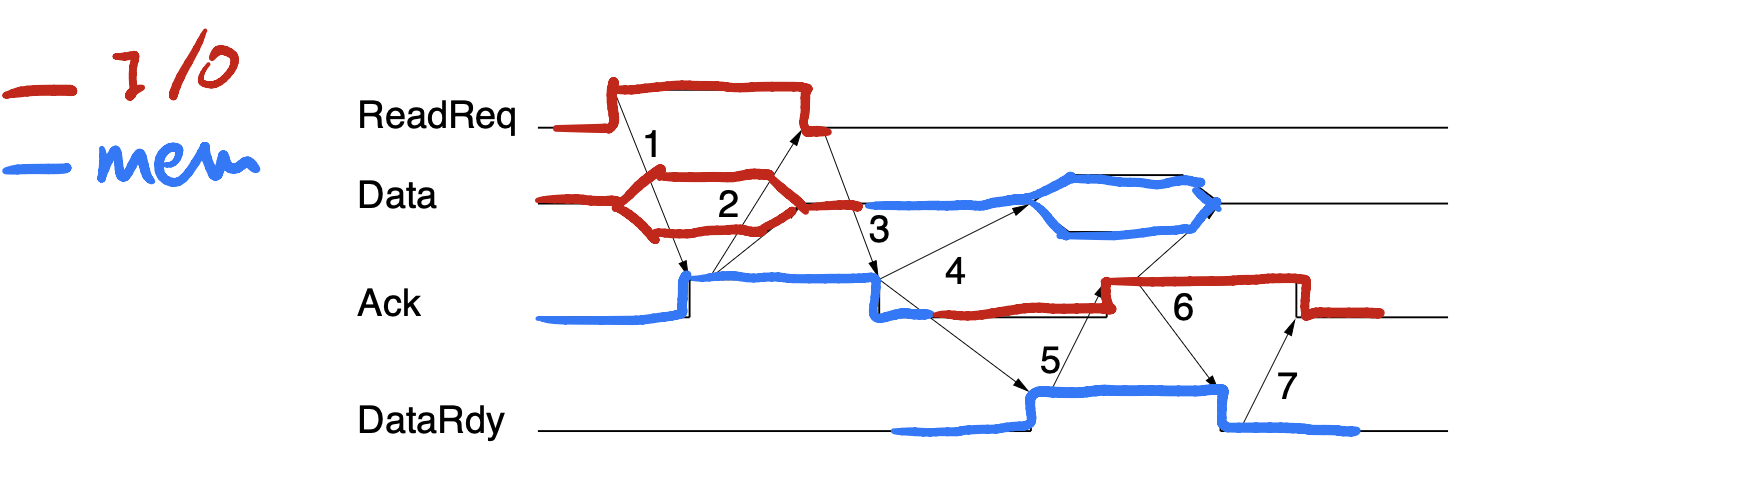
\includegraphics[width=0.7\textwidth]{figures/4F14/handshaking.png}
\end{center}
Exchange starts when the device raises ReadReq and puts address on data lines.
\begin{enumerate}
    \item Memory sees ReadReq, reads address, raises Ack.
    \item I/O sees Ack, releases ReadReq and data lines.
    \item Memory sees ReadReq low and drops Ack.
    \item When data is ready, data is put on data lines and DataRdy is raised.
    \item I/O sees DataRdy, reads data and raises Ack.
    \item Memory sees Ack, drops DataRdy and releases data lines.
    \item I/O sees DataRdy low and drops Ack.
\end{enumerate}

\textbf{I/O event presentation:}
\begin{itemize}
    \item \textit{Memory-mapped I/O:} 
    \begin{itemize}
        \item Each device appears as a set of data and control registers at a particular address.
        \item The control register contains status bits that can be continully cheked (\textit{polling}).
        \item Requires the least hardware but wasteful of CPU time.
        \item Suitable for low-bandwidth devices which can tolerate low frequency polling, e.g. mice.
    \end{itemize}
    \item \textit{Interrupt-driven I/O:} 
    \begin{itemize}
        \item An I/O device generates an interrupt when it requires attention. The CPU:
    \begin{enumerate}
        \item Stops executing the current process.
        \item Finds the cause of the interrupt.
        \item Services the interrupt.
        \item Resumes execution of the original process.
    \end{enumerate}
        \item Requires extra signal lines to interrupt the CPU.
        \item CPU must be involved in every bus transaction, but no CPU load when the device is idle.
        \item Suitable for relatively low-bandwidth devices which are mostly idle, e.g. printers.
    \end{itemize}
\end{itemize}

\textbf{Direct memory access (DMA):} Transfer data directly between memory and I/O devices without CPU involvement (the DMA controller is the bus master instead). CPU is interrupted at the start and end of each DMA.

Steps in a DMA transfer:
\begin{enumerate}
    \item The processor supply the DMA controller with: the identity of the device, the operation to perform, the source/destination memory address and the number of bytes to transfer.
    \item The DMA controller starts the transfer of the data block (may take many transactions). After each transaction, the DMA controller updates the memory read/write address.
    \item Once the DMA transfer is complete, the DMA controller interrupts the CPU, which then becomes bus master and checks that the operation completed successfully.
\end{enumerate}
(Hence the CPU is only involved at the start and end of the transfer)

DMA and virtual memory:
\begin{itemize}
    \item If the DMA controller uses physical addresses, all DMA transfer must be constrained to stay within one page.
    \item If the DMA controller uses virtual addresses, it needs to know the translations.
\end{itemize}

Problems with DMA in cache systems:
\begin{itemize}
    \item If the DMA places data directly from disk into memory, the cache may contain stale data.
    \item If the cache is write-back, the DMA unit might transfer stale data from memory to disk, bypassing the newer data in the cache.
\end{itemize}

Solutions:
\begin{itemize}
    \item Route all DMA transfers through the cache (expensive).
    \item Invalidate the cache for an I/O write or force write-backs for an I/O read (cache flushing).
    \item Selectively flush or invalidate individual caches entries for DMA.
\end{itemize}

\textbf{Buses vs point-to-point networks:} 
\begin{itemize}
    \item Clock rate of a parallel bus is limited by noise, stray capacitance, crosstalk and clock skew.
    \item To make parallel buses faster, need to make it shorter and limit the number of devices connected to it.
    \item Serial point-to-point networks mitigate the effects of different bit-wise timing skews.
    \item Serial networks can run very fast since there are only two devices on each link -- less load, noise and stray capacitance.
    \item Serial connections also require fewer wires, and does not require bus mastering protocols.
\end{itemize}
\begin{center}
    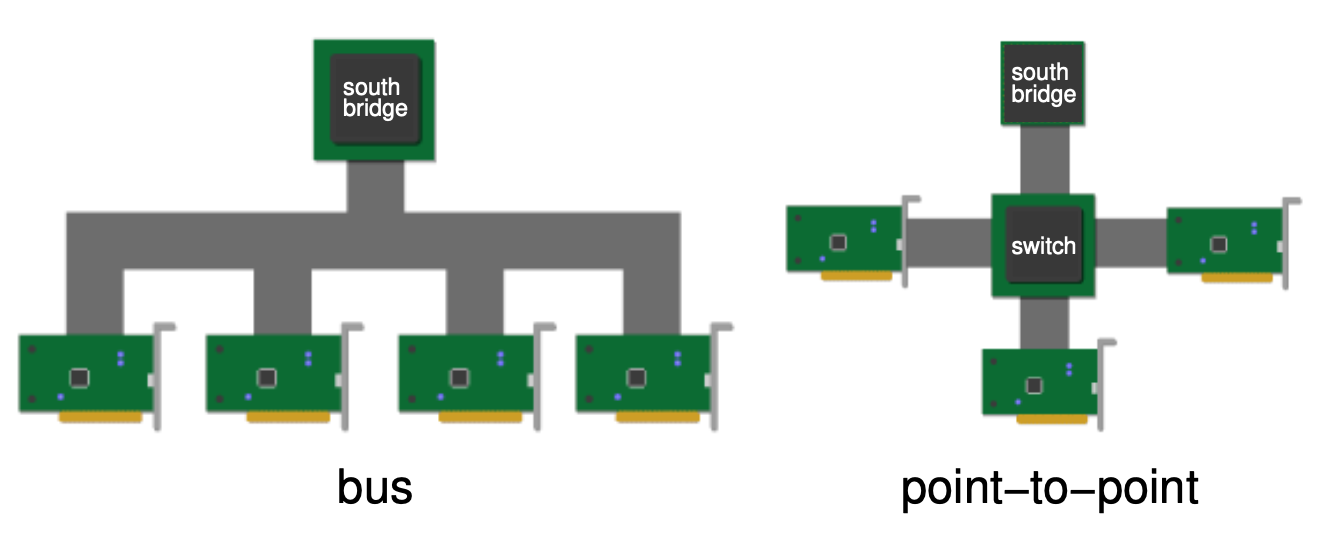
\includegraphics[width=0.6\textwidth]{figures/4F14/point-to-point.png}
\end{center}

Examples of transition from bus to network:
\begin{itemize}
    \item Parallel ATA to Serial ATA (SATA) for disks.
    \item Peripheral Component Interconnect (PCI) to PCI Express (PCIe) for generic I/O devices and graphic cards.
\end{itemize}

\section{Parallel Processing}
\textbf{Flynn's classification of parallelism:}
\begin{itemize}
    \item Single instruction stream, single data stream (SISD)
    \item Single instruction stream, multiple data stream (SIMD)
    \item Multiple instruction stream, single data stream (MISD)
    \item Multiple instruction stream, multiple data stream (MIMD)
\end{itemize}

\textbf{SIMD computers:} Operate on vectors of data. SIMD instructions are broadcast to all execution units over a network, each unit has its own registers and memory. Execution units are synchronised, each handling a different data element.

SIMD machines works best on arrays and vectors (\textit{data parallel}).

\textbf{MIMD computers:} Multiple SISD machines connected on a single bus or network. Can be used to run a separate process on each processor or a parallel processing program. The processors can communicate in two ways:
\begin{itemize}
    \item \textit{Shared memory:} All processors can access a common memory with a single address space. Communication by loads and stores. 
    
    If the memory takes the same time for all processors, it has a \textit{uniform memory access (UMA)} or \textit{symmetric multiprocessor (SMP)}. Alternative is \textit{non-uniform memory access (NUMA)}.
    \item \textit{Message passing:} Each processor has its own private memory. Slower but synchronisation is implicit.
\end{itemize}

\textbf{Challenges in developing parallel processing programs:}
\begin{enumerate}
    \item Communications overhead and/or cache issues limit speed-up.
    \item The programmers needs to know a lot about the hardware.
    \item Amdahl's law: it is not much use parallelising small parts of the program.
\end{enumerate}

\textbf{Snooping:} All cache controllers monitor the bus and react to reads and writes in other caches to ensure \textit{cache coherency}.
Two ways to deal with writes:
\begin{itemize}
    \item \textit{Write-invalidate:} the writing processor broadcasts an invalidate signal to all other caches to invalidate the copy of the block. (practical SMP systems use write-back caches with write-invalidate since it reduces bus traffic)
    \item \textit{Write-update:} the writing processor broadcasts the new data over the bus for other caches to update the copy of the block. (like a write-through cache)
\end{itemize}
On a read miss, the cache notifies other caches to check if they have a more up-to-date copy of the block.
\begin{center}
    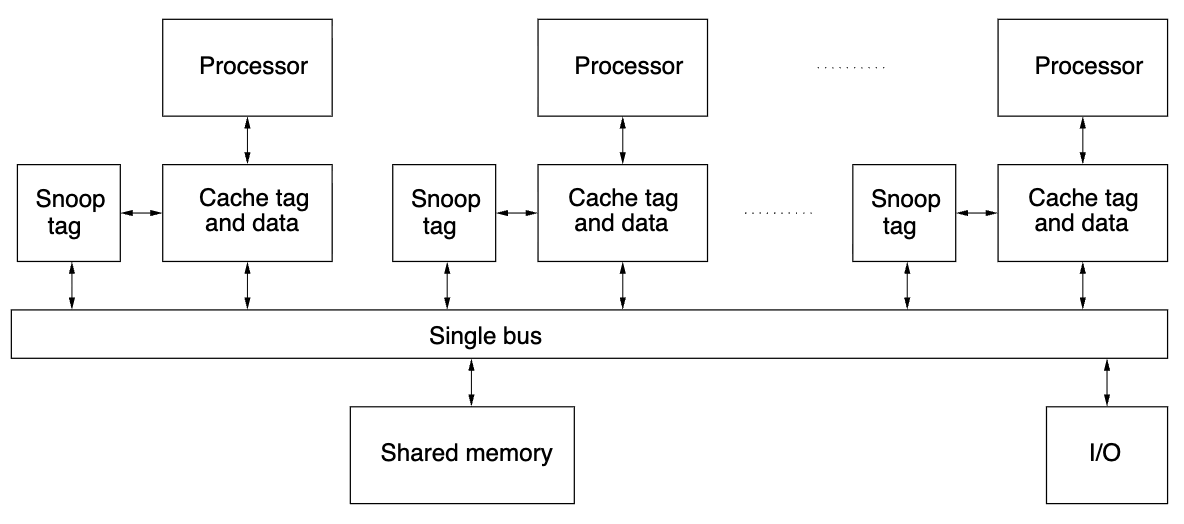
\includegraphics[width=0.6\textwidth]{figures/4F14/snooping.png}
\end{center}

\textbf{MIMD networks:}
\begin{itemize}
    \item Single bus designs are limited by the conflicting bus requirements of high bandwidth, low latency and unlimited length.
    \item Networks allow more processors than a single bus, where each processor has a local memory (\textit{distributed memory} and possibly multiple private address spaces).
    \item Alternative: NUMA with a global address space with cache coherency enforced using \textit{directories}.
\end{itemize}
\begin{center}
    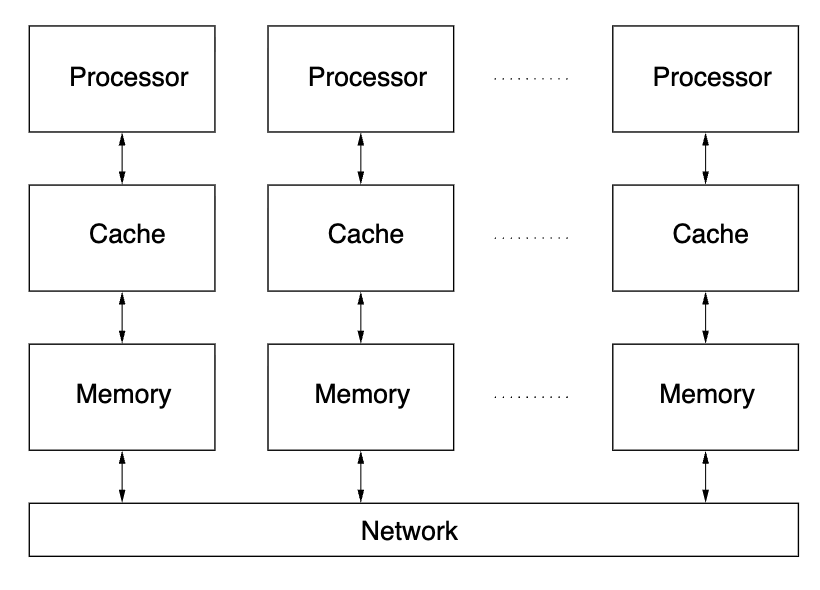
\includegraphics[width=0.4\textwidth]{figures/4F14/MIMD_network.png}
\end{center}
Networks performance can be measured by:
\begin{itemize}
    \item \textit{Total network bandwidth} = \# links $\times$ bandwidth per link (best possible performance).
    \item \textit{Bisection bandwidth:} divide the network into two and sum the bandwidth of the links crossing the division (closer to the worst case). 
\end{itemize}
Fully connected network has link between every pair of nodes, yields the best performance but is expensive. Alternatives are:
\begin{center}
    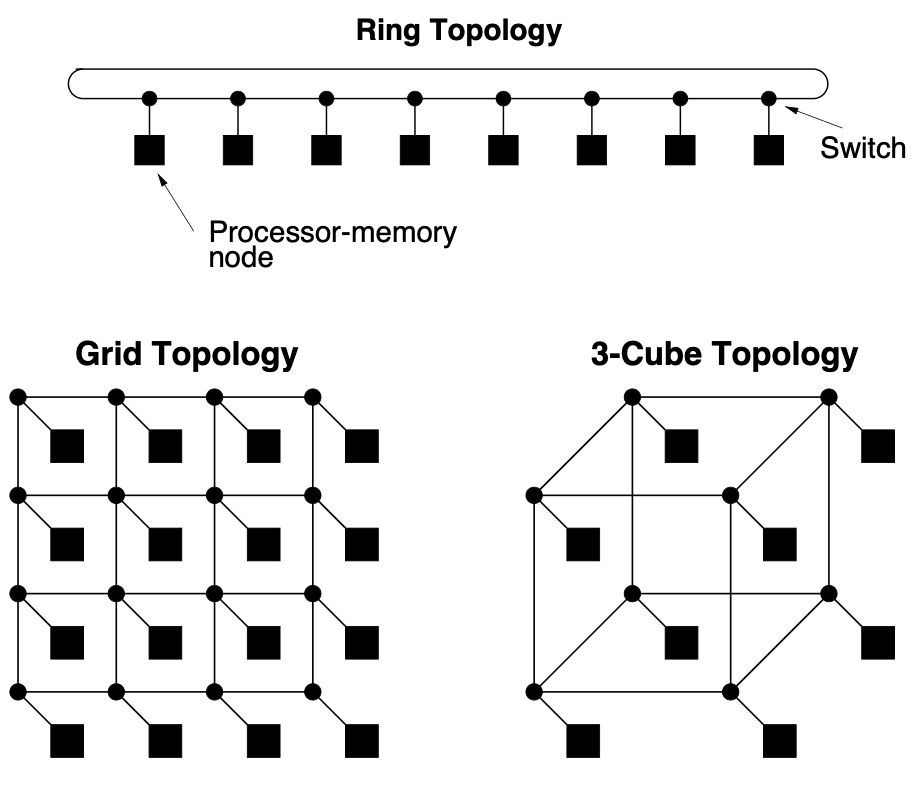
\includegraphics[width=0.4\textwidth]{figures/4F14/network_topology.png}
\end{center}

\textbf{NUMAs vs clusters:}
\begin{center}
    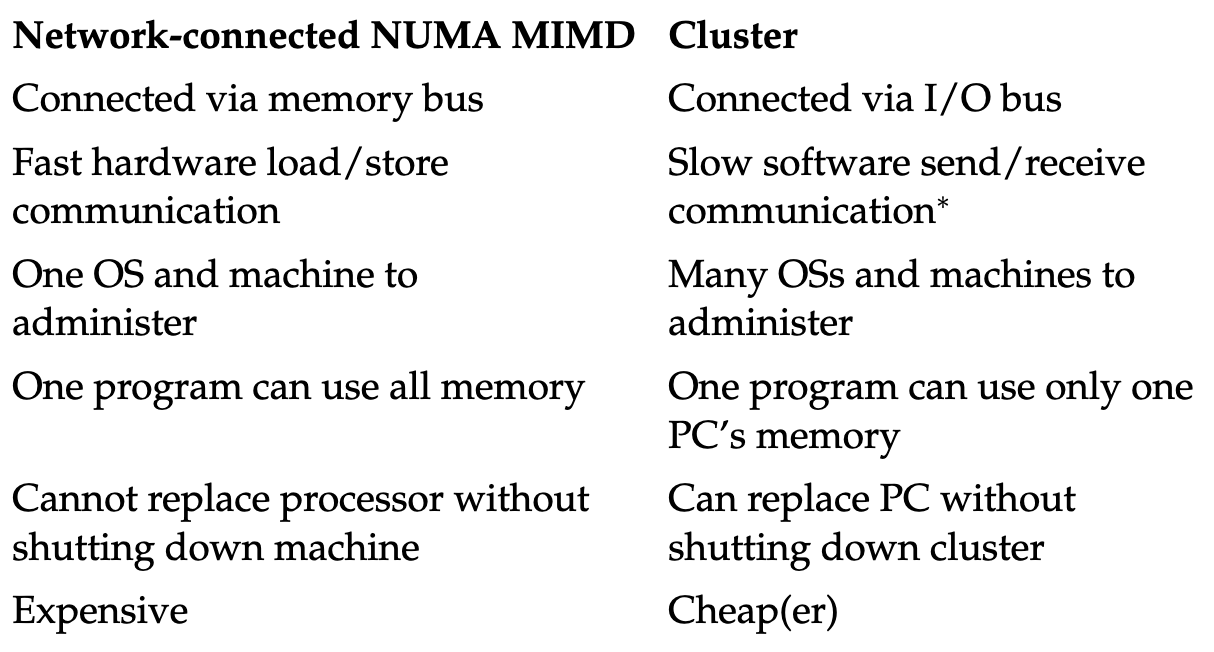
\includegraphics[width=0.6\textwidth]{figures/4F14/NUMA_vs_cluster.png}
\end{center}

\textbf{Simultaneous multithreading (SMT):} Run multiple processes concurrently on a superscalar processor. Separate register file, PC, and TLB are required for each process. ($\neq$ multi-core CPUs -- multiple entire processors on the same chip).


\end{document}